\documentclass[a4paper]{article}
\usepackage[a4paper, total={6in, 9in}]{geometry}
\usepackage{amsmath}
\usepackage{csvsimple}
\usepackage{graphicx}
\usepackage{siunitx}
\usepackage{float}
\usepackage{subcaption}
\usepackage{blindtext}
\usepackage{mathtools}
\usepackage[hidelinks]{hyperref}
\usepackage[style=iso]{datetime2}

\graphicspath{ {./img/} }

\title{Sammanfattning av Diffraktionslaboration}

\author{Emil Babayev}
\date{\today}
\begin{document}
\begin{titlepage}
	\centering
	
\includegraphics[width=0.15\textwidth]{logo.png}\par\vspace{1cm}
	{\scshape\large Lunds Tekniska Högskola \par}
	\vspace{1cm}
    {\scshape\large FAFF30 Våglära och optik\par}
	\vspace{1.5cm}
	{\huge\bfseries Sammanfattning\\Diffraktionslaboration\par}
	\vspace{2cm}
	{\Large Emil Babayev\par}
	\vfill
	Laborationshandledare\par
    Samuel Bengtsson

    \vfill
    
	{\large \today \par}
\end{titlepage}

\section{Inledning}
Länge har det diskuterats om ljuset har våg- eller partikelnatur. Diskussionen har pågått i flera hundra år och man är fortfarande inte helt överens kring vilket det är,
utan accepterar istället att ljuset uppvisar både våg- och partikelegenskaper. I denna laboration har fenomenet diffraktion(även känt som böjning) studerats, vilket är 
ett typiskt vågfenomen. Det innebär att alla resultat som åstadkommits i laborationen tyder på att ljus iallafall definitivt är en våg. Alla uppställningar har gjorts med en
röd, koherent, monokromatisk laser med våglängden $\lambda = \SI{641.3}{\nano\meter}$.

\section{Sammanfattning av laborationen}
\subsection{Fraunhoferdiffraktion}
Ljuset från lasern kollimerades och två speglar placerades i strålgången för att kunna styra strålens riktning. Den delen av laborationsbänken syns i figur \ref{fig:uppst}.
\begin{figure}[h!]
	\centering
	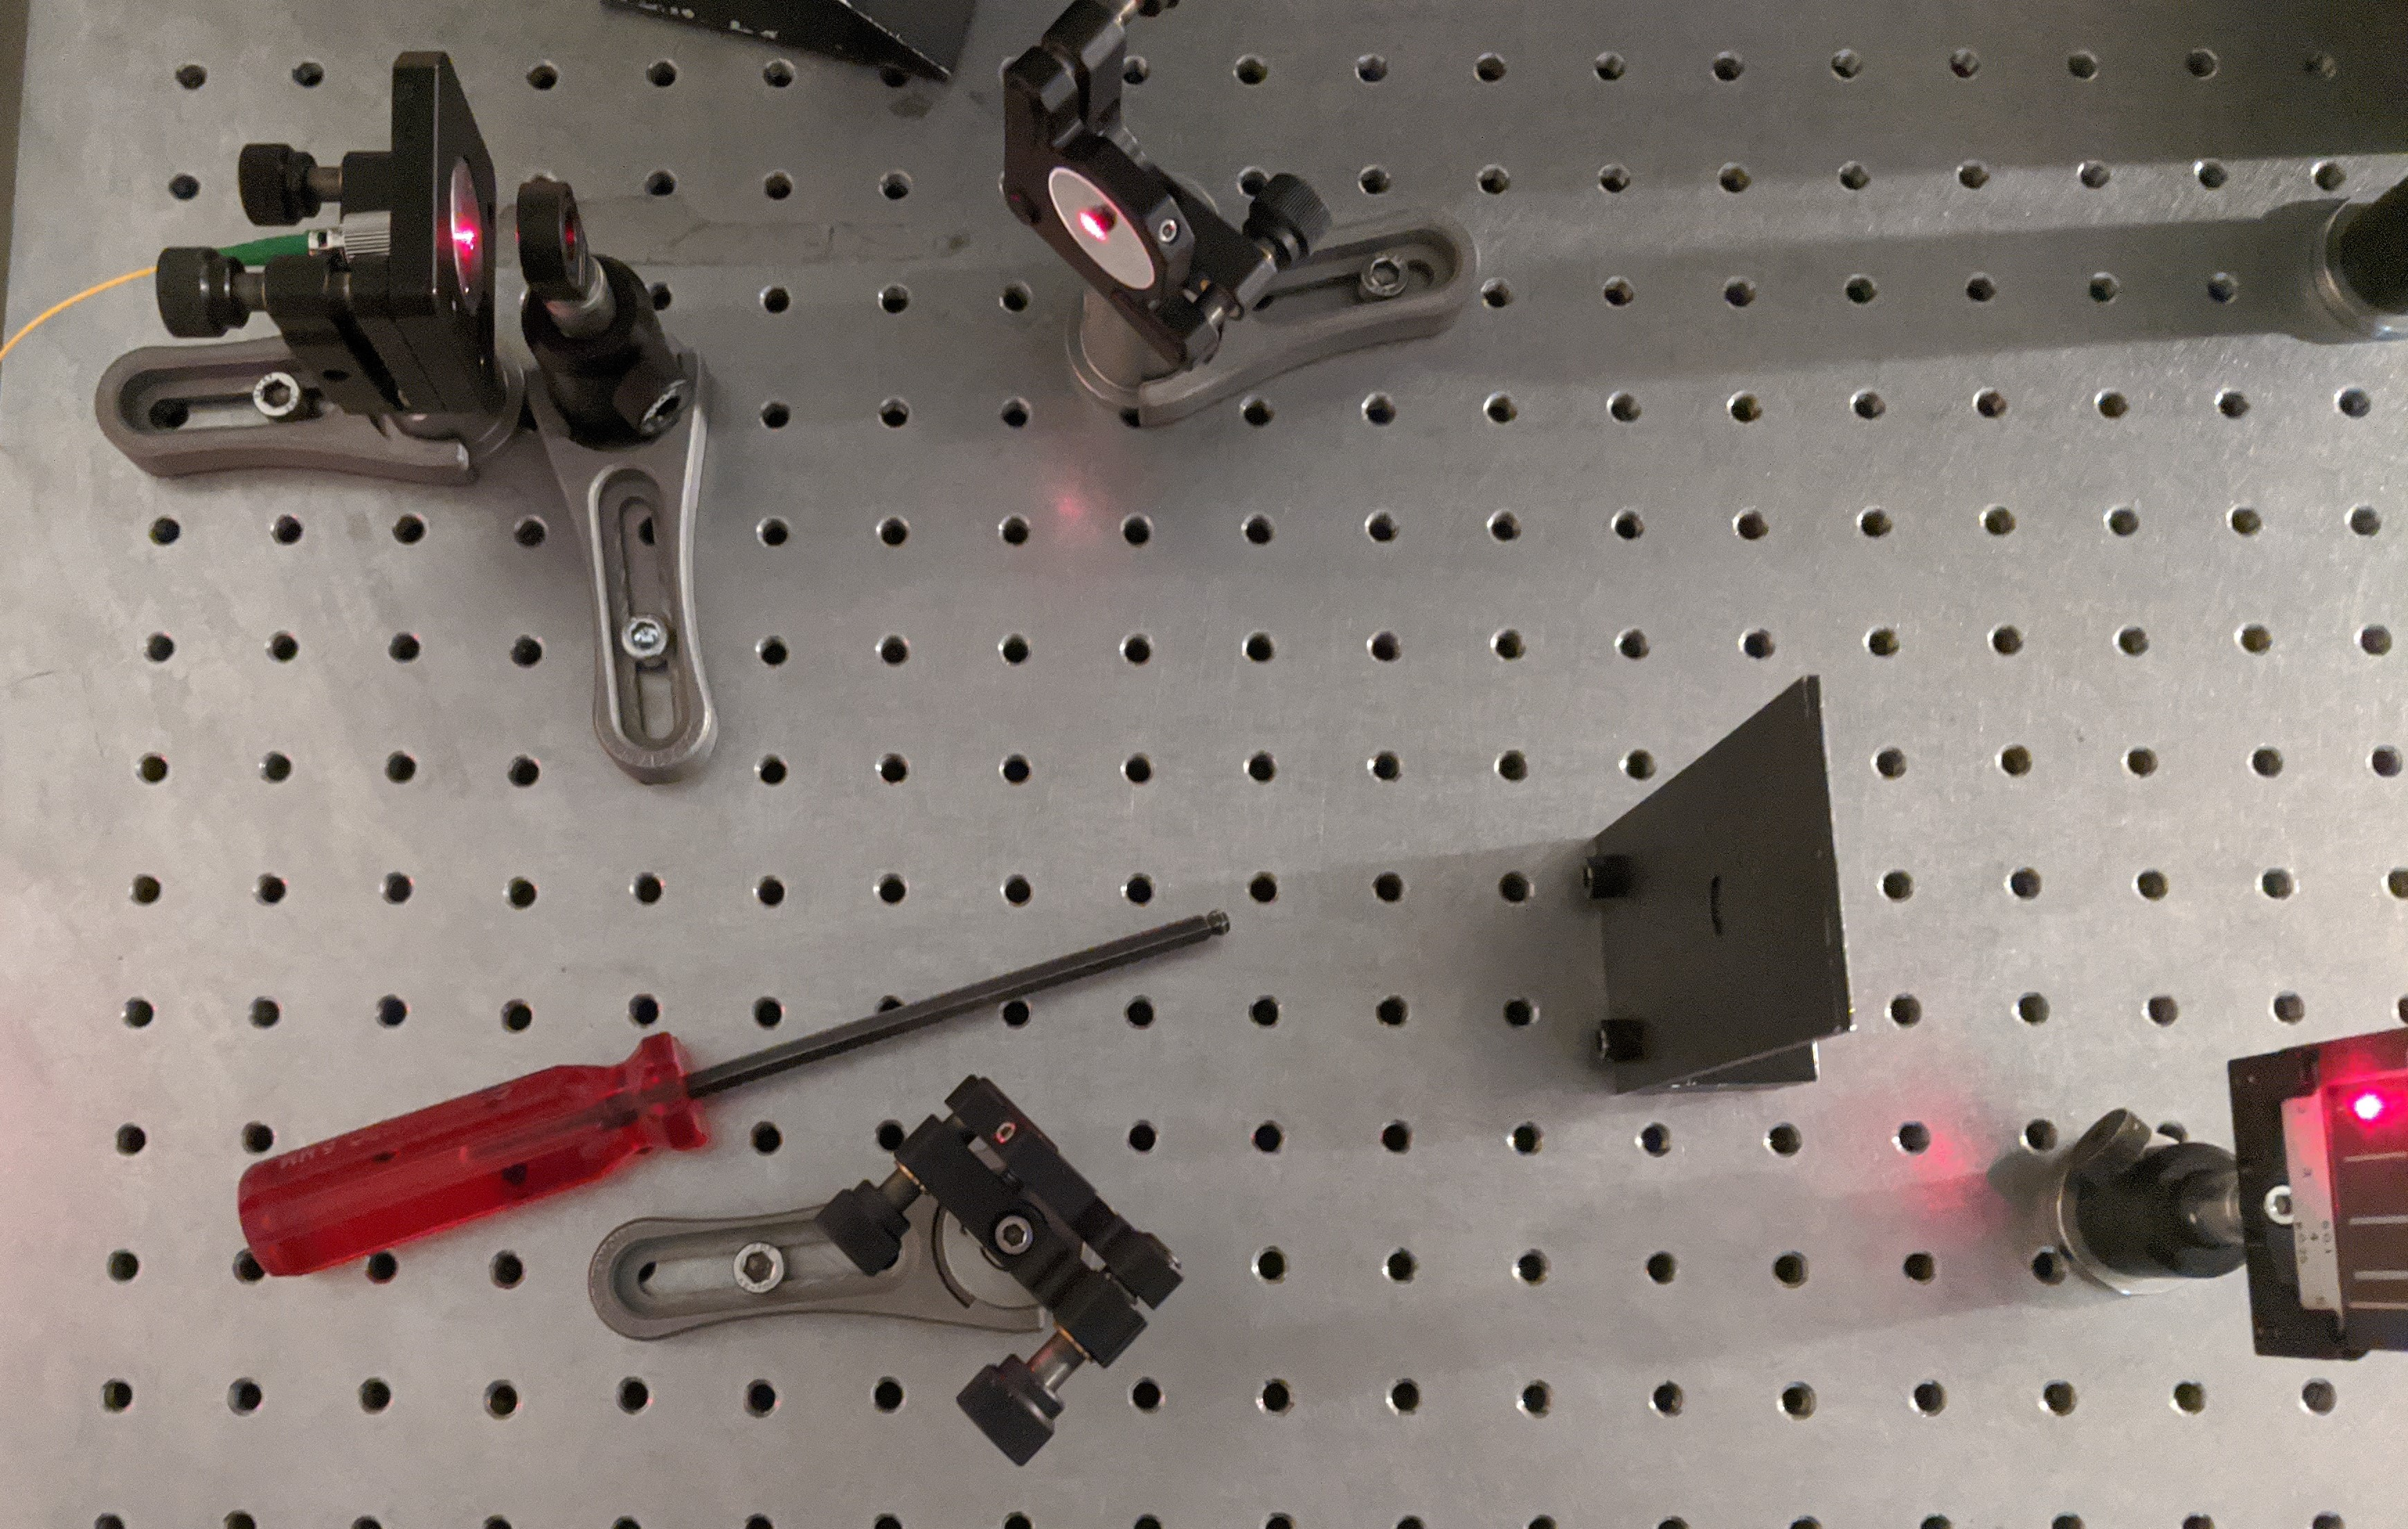
\includegraphics[width=\textwidth]{speglar.jpg}
	\caption{Labbuppställningen}
	\label{fig:uppst}
\end{figure}

\subsubsection{Dubbelspalt}
Som första delen av laborationen placerades en dubbelspalt i den kollimerade ljusstrålen. På en skärm ca 1 m längre bort iakttogs ett typiskt interferensmönster, se figur \ref{fig:dubbelspalt}.
\begin{figure}[h!]
\centering
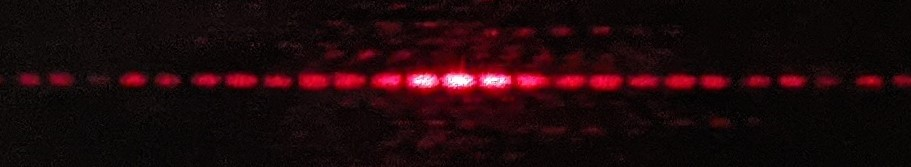
\includegraphics[width=\textwidth]{2spalt.jpg}
\caption{Interferens med dubbelspalt}
\label{fig:dubbelspalt}
\end{figure}
Uppgiften var sedan att beräkna spaltavståndet hos dubbelspalten, vilket gjordes med ekvation \ref{eq:dubbelspalt} genom att lösa ut $d$. Avståndet till skärmen mättes och ett
medelvärde togs, samt avståndet mellan två maxima av samma ordning, mätvärdena redovisas i tabell \ref{table:dubbel}. Med detta kunde spaltavståndet räknas ut, och medelvärdet
var $\SI{0.27}{\milli\meter}$.
\begin{equation}
	d sin(\theta) = m\lambda, m \in Z
	\label{eq:dubbelspalt}
\end{equation}

\begin{table}[h!]
	\begin{tabular}{|l|l|l|l|}
	\hline
	Maximats ordning (m) & Avstånd till maximum (x/cm) & Avstånd till skärmen (L/cm) & \begin{tabular}[c]{@{}l@{}}Beräknat spaltavstånd\\  (d/mm)\end{tabular} \\ \hline
	1                    & 0,24                       & 99,775                      & 0,2666                                                                  \\ \hline
	2                    & 0,5                        & 99,775                      & 0,2559                                                                  \\ \hline
	3                    & 0,65                       & 99,775                      & 0,2953                                                                  \\ \hline
	\end{tabular}
	\caption{Mätvärdena från dubbelspalten}
	\label{table:dubbel}
\end{table}
Mönstret kan förklaras genom att de två smala spalterna fungerar som punktkällor för den inkommande vågen. Dessa punktkällors vågor adderas i överallt efter spalterna, och där
väglängdskillnaden är en hel multipel av våglängden får vi maxima (vågorna interfererar i fas), och där väglängdskillnaden är en multipel av en halv våglängd fås minima 
(vågorna interfererar ur fas). Att mönstret blir svagare i kanterna beror på att även böjning sker i denna situation och fungerar som ett
"envelope" till interferensmönstret. Detta gäller för alla flerspaltsystem.

\subsubsection{Enkelspalt}
Dubbelspalten byttes ut mot en enkelspalt, och nu skulle istället spaltbredden beräknas, med hjälp av ekvationen för diffraktionsminima, ekvation \ref{eq:enkelspalt}.
Mätvärden togs, enligt tabell \ref{table:enkelspalt}. 
\begin{equation}
	b sin(\theta) = m\lambda, m \in Z
	\label{eq:enkelspalt}
\end{equation}
\begin{table}[h!]
	\begin{tabular}{|l|l|l|l|}
	\hline
	Minimats ordning (m) & Avstånd till minima (x/cm) & Avstånd till skärmen (L/cm) & \begin{tabular}[c]{@{}l@{}}Beräknad spaltbredd\\  (d/mm)\end{tabular} \\ \hline
	1                    & 0,325                      & 99,9                        & 0,1973                                                                \\ \hline
	2                    & 0,65                       & 99,9                        & 0,1973                                                                \\ \hline
	3                    & 0,95                       & 99,9                        & 0,2025                                                                \\ \hline
	4                    & 1,3                        & 99,9                        & 0,1973                                                                \\ \hline
	\end{tabular}
	\caption{Mätvärden från enkelspalten}
	\label{table:enkelspalt}
\end{table}
Mönstret som uppstod visas i figur \ref{fig:enkelspalt}. Enkelspaltens mönster förklaras på grund av fasskillnaden som
uppstår mellan alla punktkällor som skapas i spaltöppningen när de når en skärm. På vissa punkter träffar alla elementarvågor
varandra i fas (exempelvis i huvudmaximum), och på andra ställen möts de ur fas och släcker ut varandra.
\begin{figure}[h!]
	\centering
	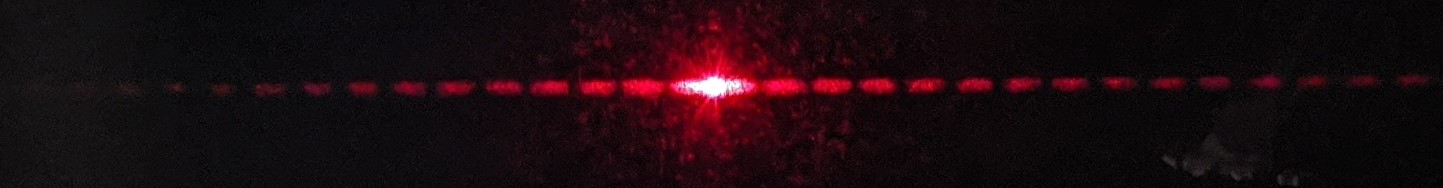
\includegraphics[width=\textwidth]{1spalt.jpg}
	\caption{Mönstret från en enkelspalt}
	\label{fig:enkelspalt}
\end{figure}
\pagebreak
\subsubsection{Babinets princip}
\begin{figure}[h!]
	\centering
	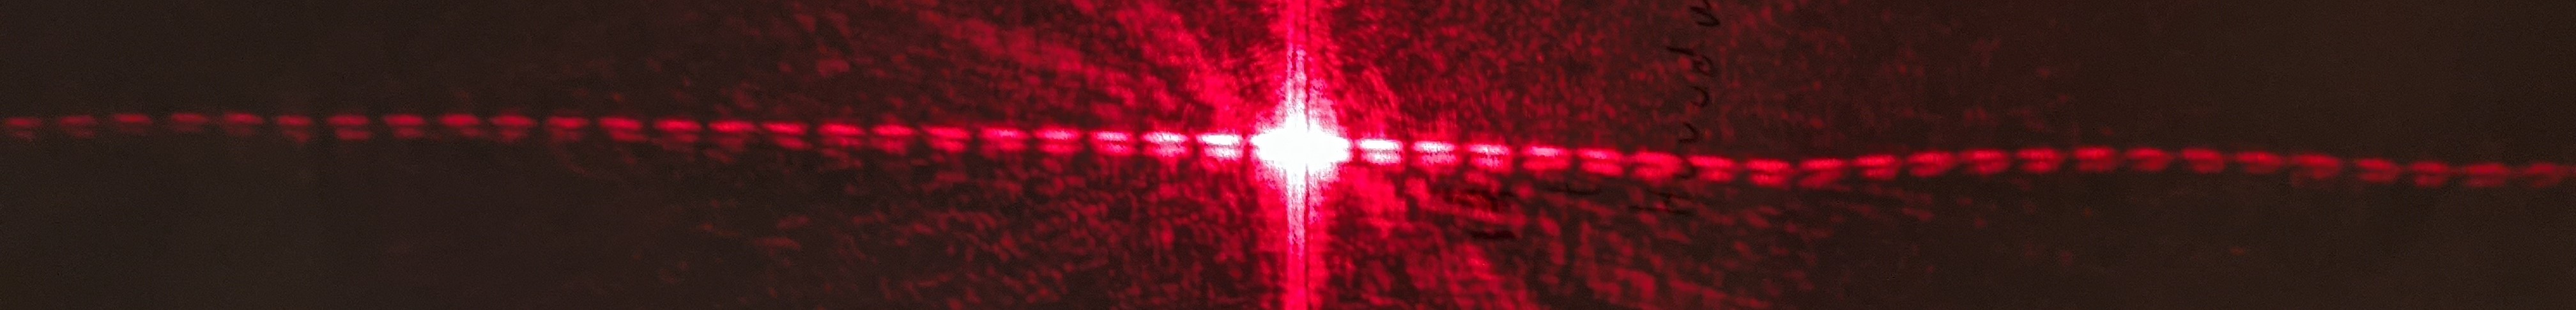
\includegraphics[width=\textwidth]{babinet.jpg}
	\caption{Två överlagrade interferensmönster i motfas}
	\label{fig:babinet}
\end{figure}
I denna del placerades strålen precis i gränsområdet mellan en tråd och spalt. Babinets princip gäller vilket innebär att
de två hindrena är komplementära och bildar samma diffraktionsmönster på skärmen. Enligt pricipen blir de två vågsystemen från
spalten respektive tråden i motfas och amplituderna släcker ut varandra där de möts. Eftersom hindrena är komplementära kan man tänka
sig att kombinationen av de två inte borde leda till något ljus alls (alltså att det skulle bli mörkt om en spalt och tråd placerades på samma ställe)
vilket också förklarar fenomenet.
\subsubsection{Flerspaltsystem}
\begin{figure}[h!]
	\centering
	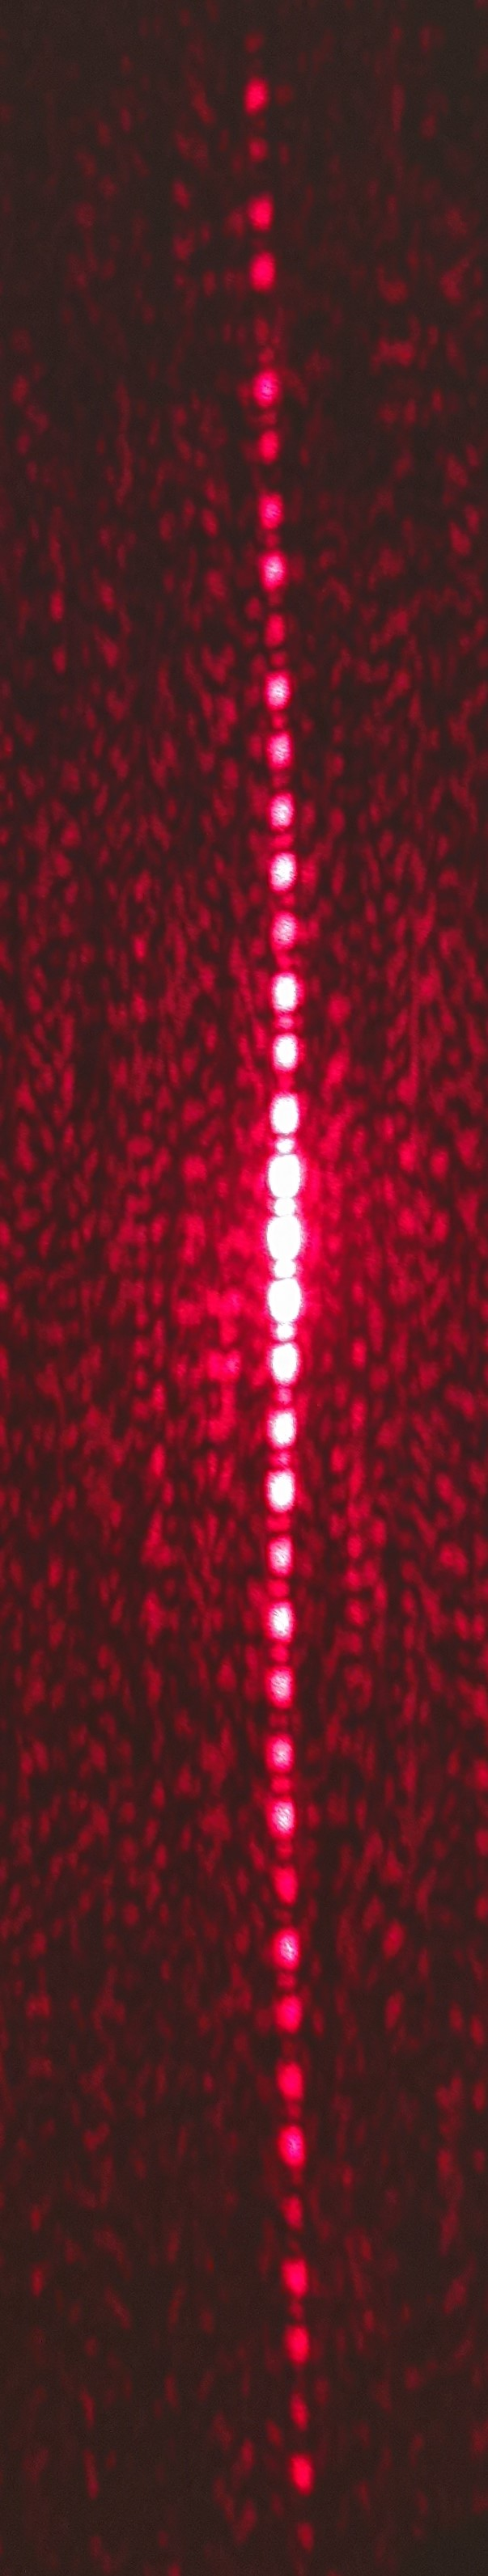
\includegraphics[width=0.17\textwidth, angle=90]{3spalt.jpg}
	\caption{Ett trespaltssystem, ett bimax syns tydligt}
	\label{fig:3spalt}
\end{figure}

\begin{figure}[h!]
	\centering
	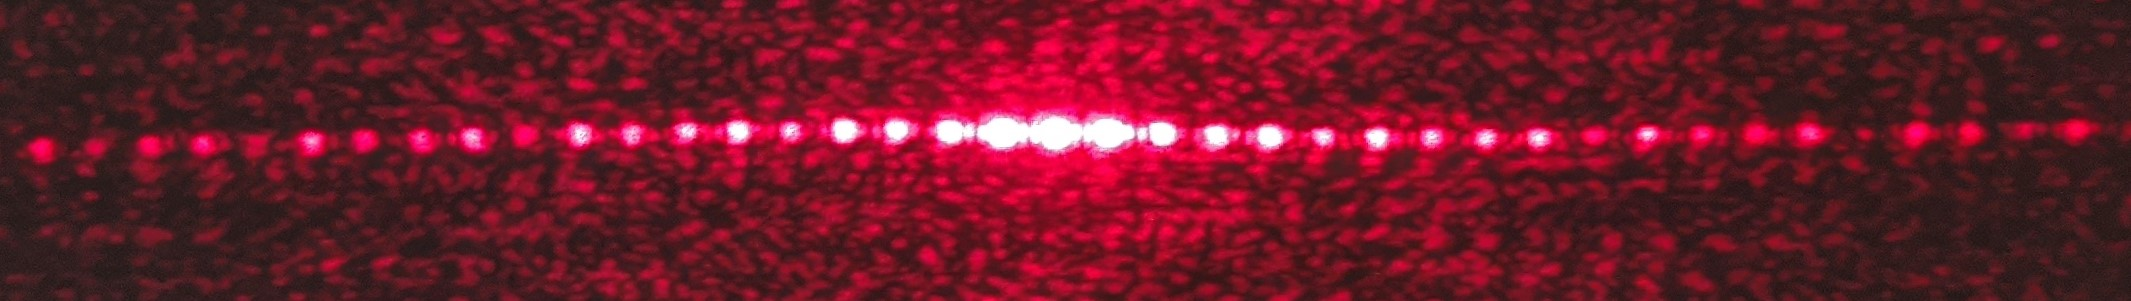
\includegraphics[width=\textwidth]{4spalt2.jpg}
	\caption{Ett fyrspaltssystem, två bimax är urskiljbara}
	\label{fig:4spalt}
\end{figure}
\begin{figure}[h!]
	\centering
	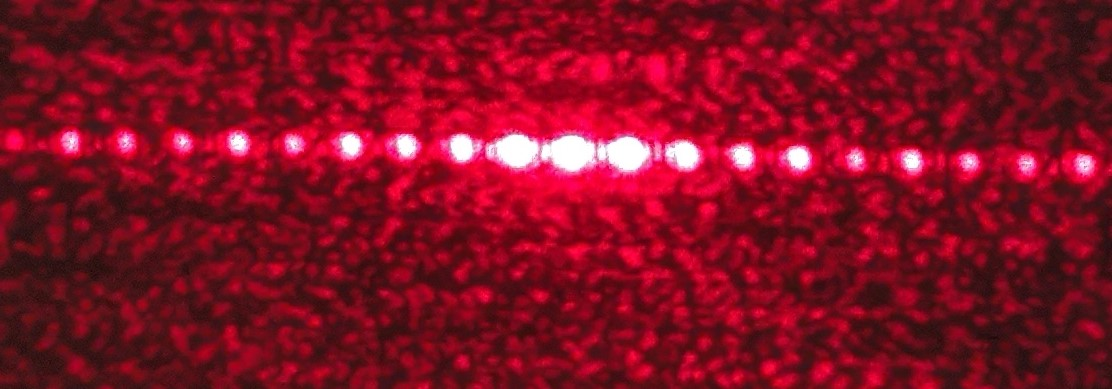
\includegraphics[height=0.1\textheight]{5spalt.jpg}
	\caption{Ett femspaltssystem, tre bimax är urskiljbara}
	\label{fig:5spalt}
\end{figure}
Därefter placerades ett tre-, fyr- och femspaltssystem i ljusstrålen. Även dessa system vållar interferensmönster (likt dubbelspalten, figur \ref{eq:dubbelspalt}) 
mellan punktkällor, men eftersom vi ökar antalet källor uppstår även andra intressanta bieffekter. Vi behåller de ljusaste maxima, som nu kallas huvudmaxima, på
samma plats, men de blir ljusare och smalare ju fler spalter vi har. Att de blir smalare måste innebära att de blir ljusare eftersom energin måste ta vägen någonstans.
Den största skillnaden är att här även uppstår bimaxima, ljusa fläckar mellan huvudmaxima. Detta beror på att fasskillnaden mellan de inkommande vågorna blir sådan att vissa vågor släcker ut varandra, men inte alla. Därför når fortfarande en del av 
intensiteten fram. Där vågorna råkar vara helt i motfas får vi återigen minima, men de blir fler. Vi får $N-2$ bimax och $N-1$ minima, där $N$ är antalet spalter.
Detta är alltså antalet fasförskjutningar mellan elementarvågorna som råkar skapa (delvis) utsläckning. 

Dessa effekter kan iakttas i figurerna \ref{fig:3spalt}, \ref{fig:4spalt} och \ref{fig:5spalt}. 
\subsection{Fresneldiffraktion}
När den kollimerande linsen sedan tas bort från ljuskällan så att den blir divergent kan man iaktta Fresneldiffraktion. Den
analytiska modellen är något avancerad(kräver en del vektoraddition) så jag förutsätter en konceptuell förståelse. 
\subsubsection{Ställbar spalt}
\begin{figure}[h!]
	\centering
    \begin{tabular}{cc}
    \subfloat[Liten spaltbredd, fraunhoferdiffraktion]{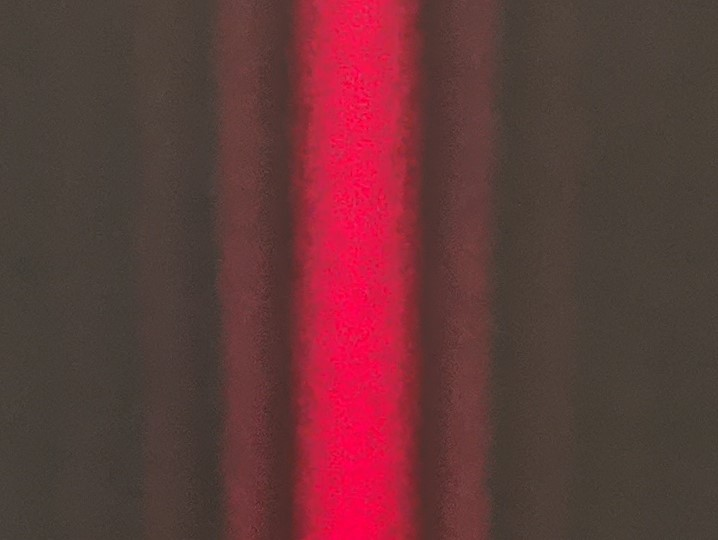
\includegraphics[width = 2.5in]{fraunhofer.jpg}} &
    \subfloat[Spaltbredden ökar tills det uppstår ett minimum i mitten]{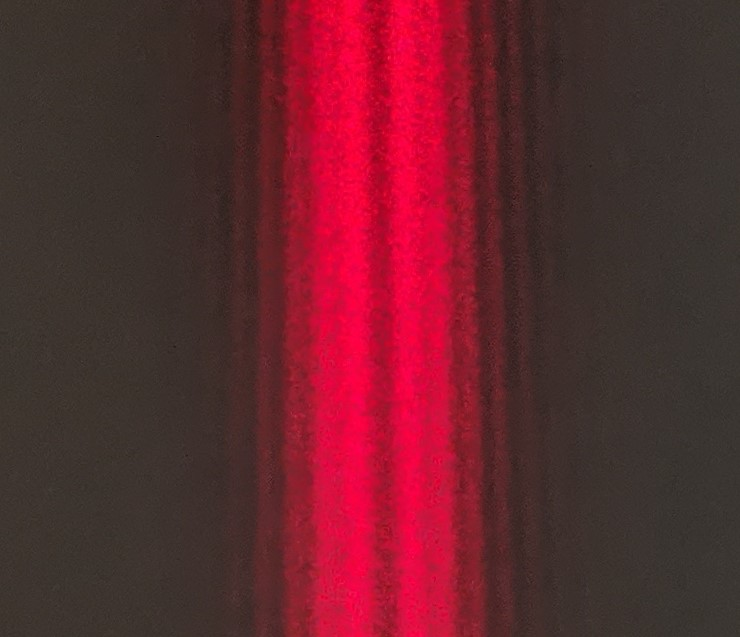
\includegraphics[width = 2.5in]{fresnel.jpg}}\\
    \subfloat[Ytterligare bredd skapar ett annat mönster]{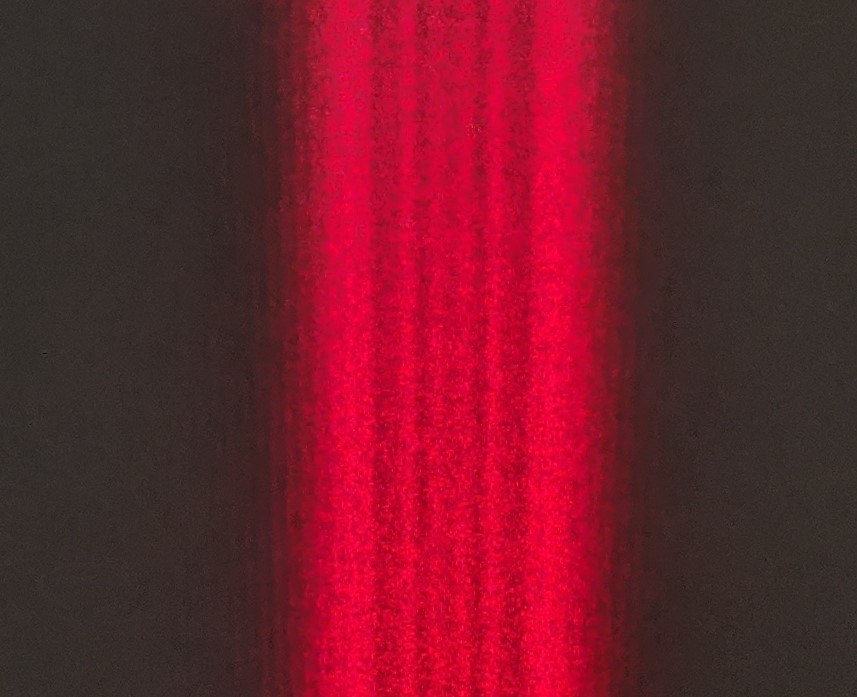
\includegraphics[width = 2.5in]{bigfresnel.jpg}} &
    \subfloat[Ännu bredare]{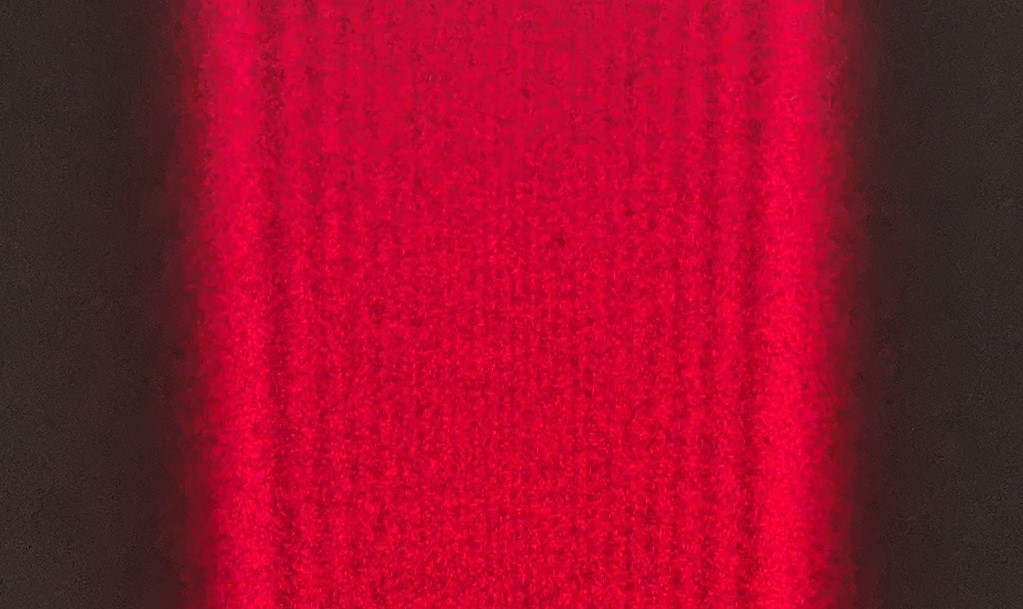
\includegraphics[width = 2.5in]{biggerfresnel.jpg}}\\
    \end{tabular}
    \caption{övergång mellan fraunhofer- och fresneldiffraktion}
    \label{fig:fresnel}
\end{figure}
Med en ställbar spalt kunde man återskapa både fraunhofer- och fresneldiffraktion. När spaltbredden är liten (figur \ref{fig:fresnel}a) är de inkommande vågorna så gott som parallella
och spalten är tillräckligt liten för att det skall uppstå fraunhoferdiffraktion. Vi har ett huvudmaximum i mitten. När spaltbredden sedan ökar övergår maximat till ett minimum, och det 
är analytiskt omöjligt för fraunhoferdiffraktion, alltså måste man då övergått till fresneldiffraktion, se figur \ref{fig:fresnel}b. När spalten sedan öppnas mer blir diffraktionsmönstret bredare och fler "toppar
och dalar" uppstår, se figurer \ref{fig:fresnel}c och d.
\pagebreak
\subsubsection{Rak kant}
\begin{figure}[h!]
	\centering
    \begin{tabular}{cc}
    \subfloat[Kanten nära skärmen, inget urskiljbart mönster]{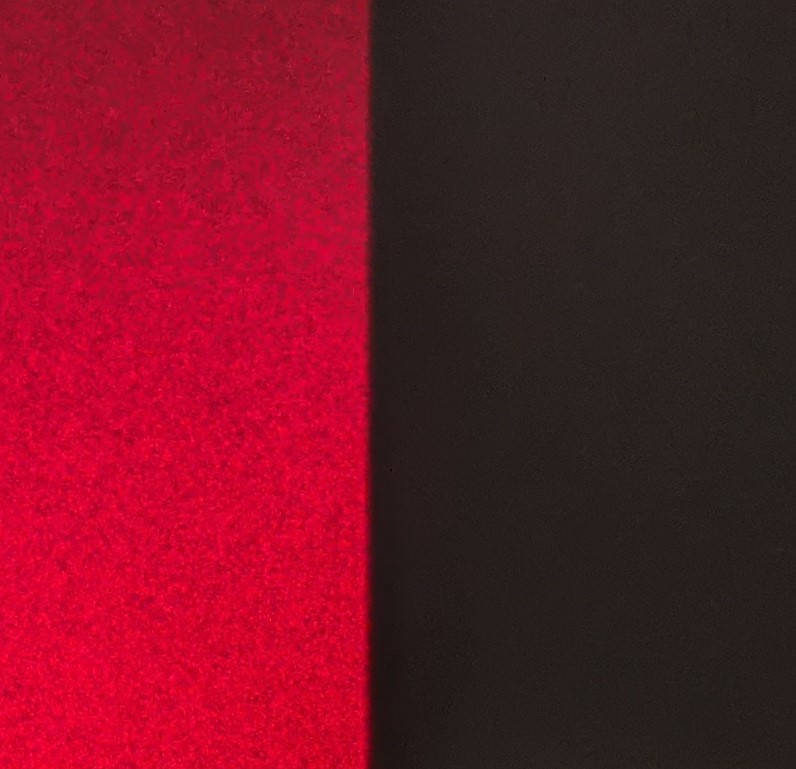
\includegraphics[width = 2.5in]{rakkant1.jpg}} &
    \subfloat[Svagt interferensmönster uppstår]{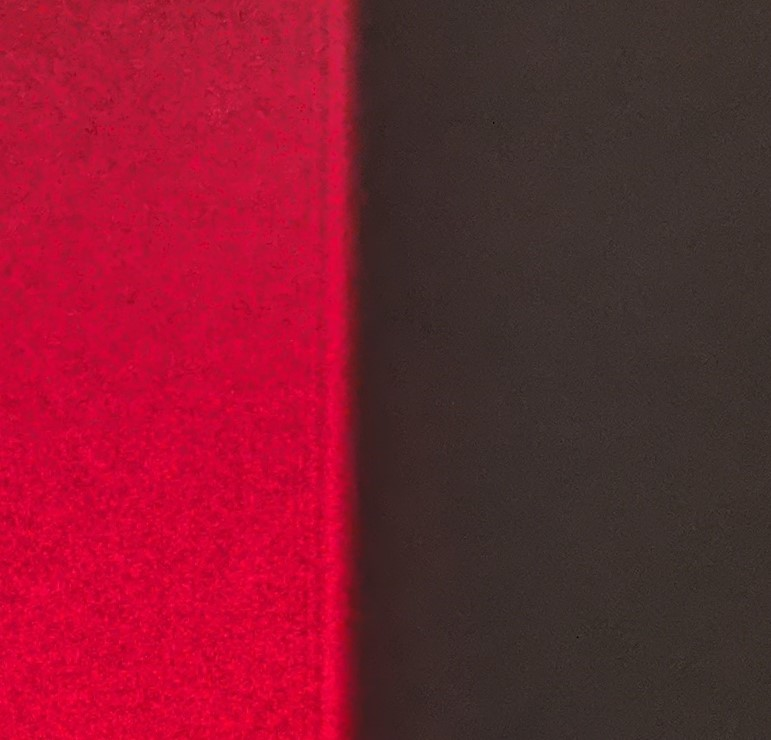
\includegraphics[width = 2.5in]{rakkant2.jpg}}\\
    \subfloat[Ju närmare kanten förs till ljuskällan, ju tydligare blir effekten]{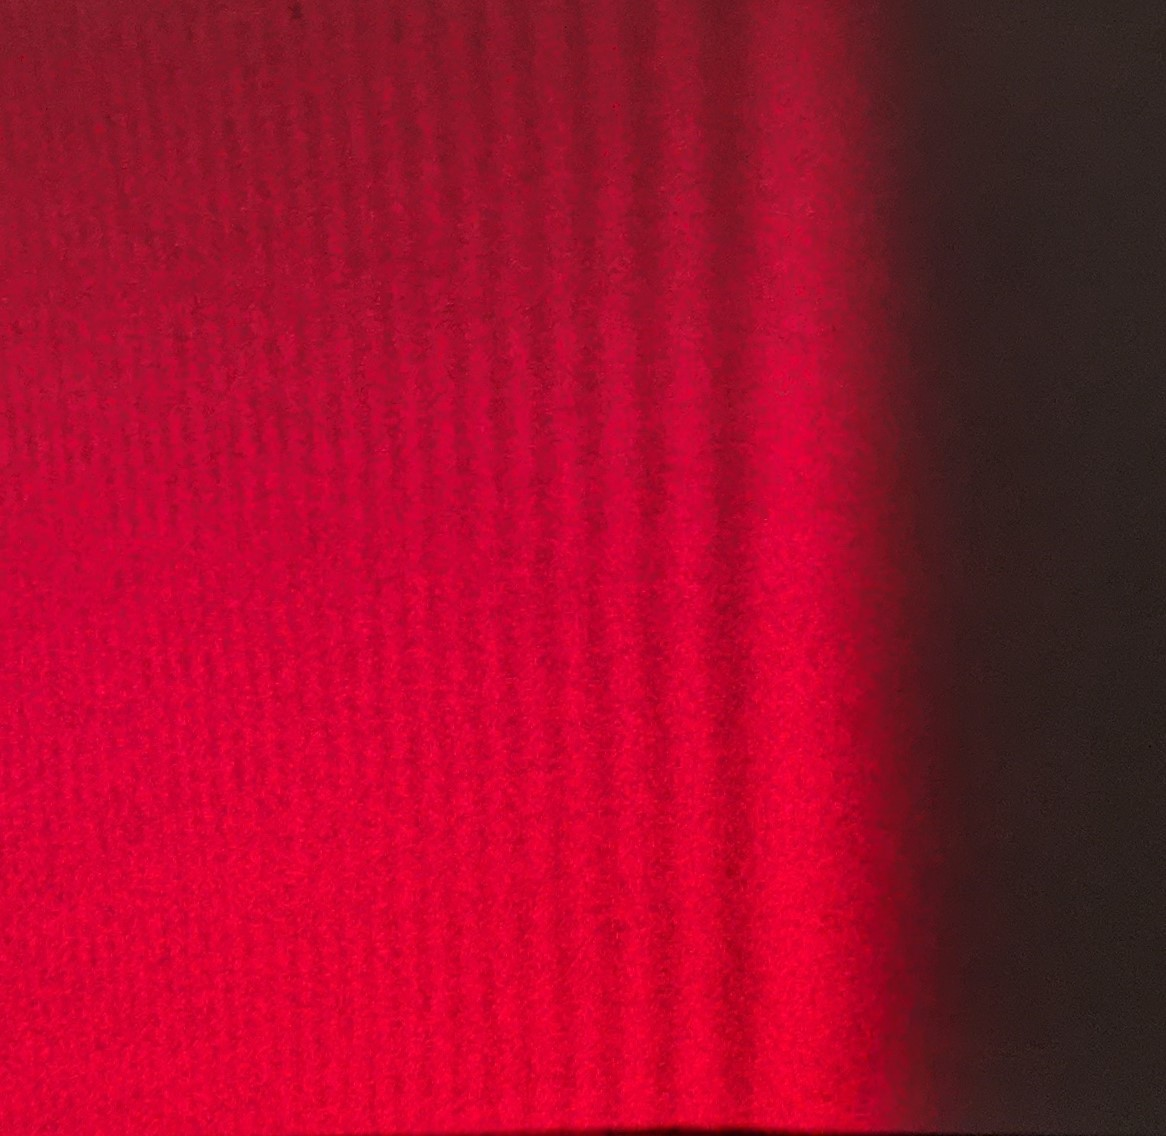
\includegraphics[width = 2.5in]{rakkant3.jpg}} &
    \end{tabular}
    \caption{Fresneldiffraktion mot rak kant}
    \label{fig:rakkant}
\end{figure}
Med en rak kant kan också fresneldiffraktion iakttas. När kanten placeras framför den divergenta strålen, nära skärmen kan inget diffraktionsmönster
iakttas (figur \ref{fig:rakkant}a). När man sedan för kanten närmare ljuskällan minskar parallelliteten hos ljusstrålarna och en mer påtaglig
fresneldiffraktion kan iakttas, figurer \ref{fig:rakkant}b och c.

Ett sådant här mönster uppstår mot en rak kant eftersom ljuset böjs även här. Man ser också i bilderna att ljuset böjs runt kanten och in i det område
som är mörkt under vanliga omständigheter (syns tydligast i \ref{fig:rakkant}c) och högerkanten på bilderna är därför lite "mjuk". På den vänstra sidan
uppstår vanlig fresneldiffraktion, främst med vågorna som böjs av kanten, och det är detta som leder till den vågaktiga intensitetsfördelningen på vänster
del av skärmen. Detaljerna av hur ljuset böjs runt en rak kant har jag inte direkt koll på.
\pagebreak
\subsubsection{Hål}
I denna del skulle diametern på ett hål bestämmas med hjälp av fresneldiffraktion. Detta görs genom att först placera hålet
nära skärmen (så att fraunhoferdiffraktion uppstår då vi har så gott som parallella strålar, figur \ref{fig:fresnel}a) och sedan flytta hålet närmare ljuskällan
tills det uppstår ett minimum i mitten av mönstret, figur \ref{fig:fresnel}b. Första gången detta uppstår kan man vara säker på att vi hade två fresnelzoner, då
är fasskillnaden mellan mitten av hålet och översta kanten en hel våglängd och ljuset släcks ut helt i mitten. När hålet sedan flyttas närmare ljuskällan blir centrum
av skuggan alternerande ljus och mörk, och man vet att man nått nästa fresnelzon. Tre fresnelzoner ger ljus prick i mitten (figur \ref{fig:fresnel}c) och fyra ger återigen
mörk, då fasskillnaden är en hel multipel(2) av våglängden (figur \ref{fig:fresnel}d).
\begin{figure}[h!]
	\centering
    \begin{tabular}{cc}
    \subfloat[Inkommande strålar parallella, fraunhoferdiffraktion]{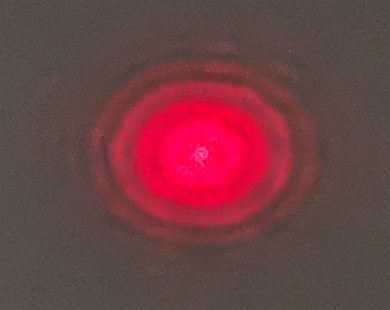
\includegraphics[width = 2.5in]{cirkel_f.jpg}} &
    \subfloat[Två fresnelzoner]{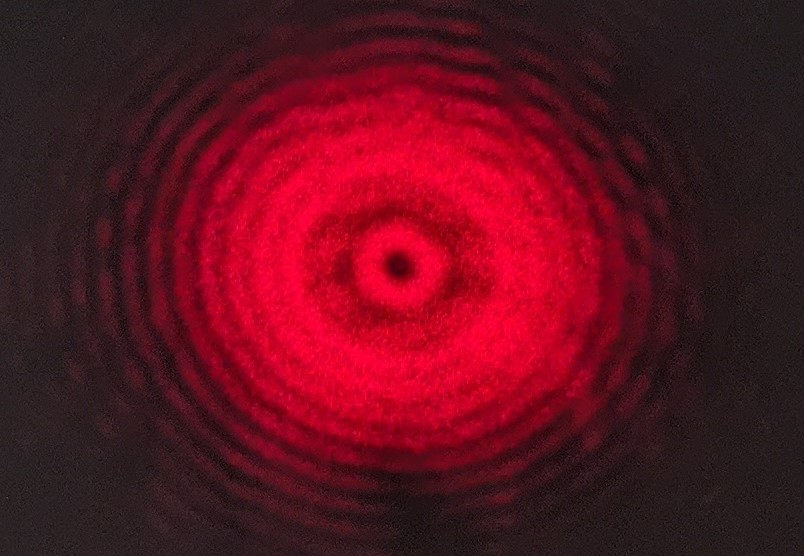
\includegraphics[width = 2.5in]{cirkel_fresnel1.jpg}}\\
    \subfloat[Tre fresnelzoner]{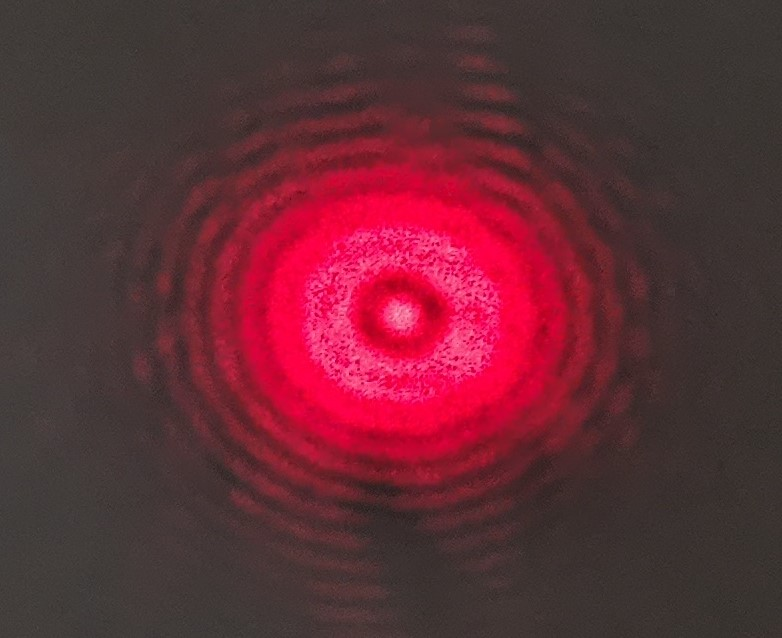
\includegraphics[width = 2.5in]{cirkel_fresnel2.jpg}} &
    \subfloat[Fyra fresnelzoner]{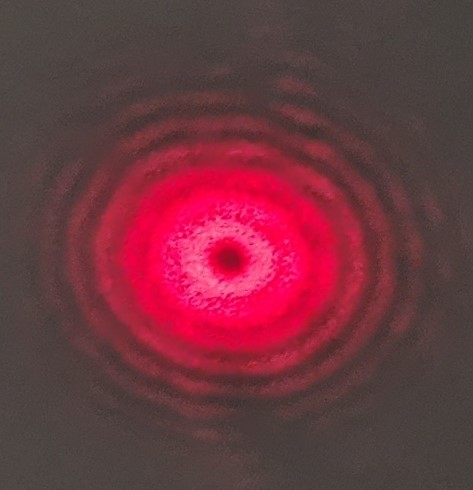
\includegraphics[width = 2.5in]{cirkel_fresnel3.jpg}}\\
    \end{tabular}
    \caption{Övergång mellan fraunhofer- och fresneldiffraktion}
    \label{fig:fresnel}
\end{figure}
För att sedan beräkna hålets diameter används pythagoras sats tillsammans med kunskapen om fasskillnaden (och fresnelzonerna).
För varje fresnelzon mättes avståndet till ljuskällan och samband \ref{eq:hole} ställdes upp, utifrån figur \ref{fig:fasskillnad}, 
med beteckningar enligt tabell \ref{tab:hole}. $m$ är hur många multiplar av våglängden vi har i fresnelzonen, alltså antalet fresnelzoner/2.
\begin{equation}
	(L + m\lambda)^2 = r^2 + L^2
	\label{eq:hole}
\end{equation}

\begin{table}[h!]
	\centering
	\begin{tabular}{|l|l|l|}
	\hline
	Fasskillnad $\lambda$/m & Avstånd till hålet (L/cm) & Beräknad hålradie (r/mm) \\ \hline
	1                                 & 7,76                      & 0,3153                   \\ \hline
	1,5                               & 5,05                      & 0,3117                   \\ \hline
	2                                 & 3,60                      & 0,2996                   \\ \hline
	\end{tabular}
	\caption{Mätvärden från hålet}
	\label{tab:hole}
\end{table}
$r$ beräknades ur mätvärdena med hjälp av ekvation \ref{eq:hole} och vi fick ett medelvärde på $r=\SI{0.30}{\milli\meter}$, alltså
en hålradie på $\SI{0.6}{\milli\meter}$, vilket bedömdes som rimligt.
\begin{figure}
	\centering
	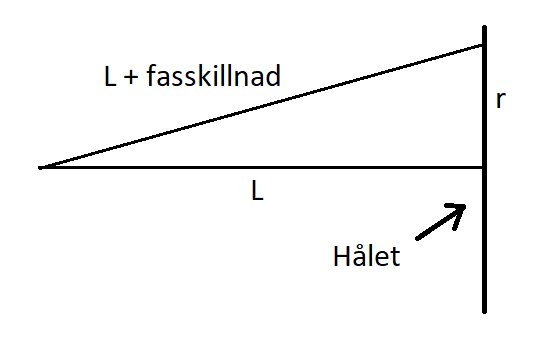
\includegraphics[width=0.5\textwidth]{fasskillnad.png}
	\caption{Sambandet för att beräkna hålets radie}
	\label{fig:fasskillnad}
\end{figure}
\subsubsection{Aragos fläck}
Tyvärr glömde jag ta en bild på Aragos/Poissons fläck, men den är inte särskilt svår att beskriva.

När man belyser ett cirkulärt hinder uppstår ett intressant fenomen, det blir nämligen en liten ljus prick i mitten av skuggan från hindret.
Detta kan också förklaras med böjning. När ljuset böjs runt det cirkulära hindret följer även lite intensitet med bakom hindret. Just i mitten
av skuggan möts alla vågor i fas (väglängdskillnaden är noll), och därför blir det konstruktiv interferens just i mitten av skuggan.

\end{document}
